\documentclass[10pt,a4paper]{scrartcl}
\pagestyle{empty}
\usepackage{a4} % alternativ \usepackage{a4wide}
\usepackage[utf8]{inputenc} % Unicode
\usepackage[ngerman]{babel} % Neudeutsche Silbentrennung (mehrsprachiges Dokument)
\usepackage{parskip} % Skip indentation of first row
\usepackage{graphicx} % Graphics support
\usepackage{longtable} % Tables across several pages
\usepackage{hyperref} % Hyperlinks
\usepackage[automark]{scrpage2} %kopf/fusszeile

\linespread{1.3}

\author{Danilo Bargen, Christian Fässler, Jonas Furrer} 
\title{Evaluation Datenbank\\Projekt BierIdee}

\pagestyle{scrheadings}
\ihead{SE2 Projekte} %linke Kopfzeile
\ohead{BierIdee} %rechte Kopfzeile

\begin{document}

\begin{titlepage}
	\maketitle
	\vspace{120mm}
	\thispagestyle{empty} % Don't start page numbers on this page
\end{titlepage}

\section{Evaluation}

\subsection{Vorwort}

Da es sich beim Projekt BierIdee - im Rahmen des Modules Software Engineering 2 Projekte - um ein
Projekt mit stark beschränktem Zeitbudget handelt und zudem der Fokus auf der Anwendung des
\textit{Rational Unified Process} liegt, wird diese Evaluation bewusst einfach gehalten. Die
Produkt-Auswahl enthält auch subjektive Kriterien, da die Zeit für eine ausgwogene objektive
Beurteilung fehlt.

\subsection{Einführung}

Es stellt sich die Frage, wie sich unsere Problemdomain -- die Bierempfehlungen -- am besten
modellieren lässt. Zwei Ansätze die sich herauskristalisiert haben sind Vektorräume und Graphen.

\subsection{Verfahren}

Zur Auswahl stehen zwei Verfahren: Vektorräume und Graphen. Diese Auswahl entstand
sowohl durch eine Besprechung mit einem Mathematik-Dozenten wie auch durch
eigenständige Recherchen.

\subsubsection{Vektorräume mit relationaler Datenbank}

Bei der Modellierung mittels Vektorräumen werden die Bewertungen der Biere mittels Vektoren
dargestellt. Jede Vektorkomponente stellt dabei ein Bier dar.

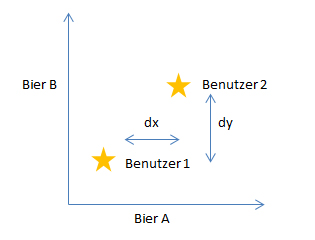
\includegraphics[scale=1]{vektor.jpg} 

Möchte man nun für einen Benutzer A eine Empfehlung erstellen, vergleicht man alle Bewertungen des
gleichen Bieres der anderen Benutzer (selbe Vektorkomponente). Danach "`erforscht"' man die anderen
Bierbewertungen der anderen Benutzer (restliche Vektorkomponenten). Um eine hohe
Empfehlungsgenauigkeit zu erhalten, ist eine sehr aufwendige Aggregierung sämtlicher Konsumationen
notwendig.

\subsubsection{Graphen mittels Graphen-Datenbank}

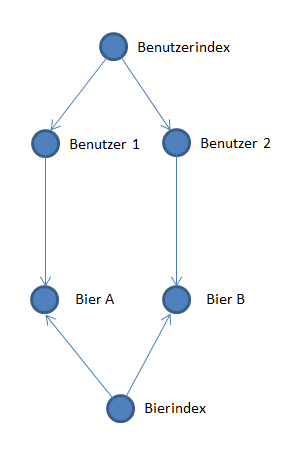
\includegraphics[scale=0.7]{graph.jpg} 

In einer Graphdatenbank werden die Benutzer und Biere mittels Knoten in einem Graph
modelliert. Die Konsumationen und Bewertungen werden mittels Kanten
(Beziehungen) zwischen den Benutzern und Bieren dargestellt. Möchte man nun einem
Benutzer eine Empfehlung aufgrund einer Konsumation machen, lässt
sich das sehr einfach bewerkstelligen, indem man über andere Nutzer "traversiert", die
das selbe Bier ebenfalls konsumiert haben.

Beispiel: $$\texttt{Benutzer 1 -- [:Konsumiert] - > Bier A < - [:Konsumiert] -- Benutzer 2}$$

\subsection{Beispielfall}

Es soll eine Empfehlung für einen Benutzer 1 erstellt werden. Die Empfehlung soll auf den bereits
konsumierten Bieren (Bier A) basieren. Es soll ein bisher vom Benutzer 1 noch nicht konsumiertes
Bier B gefunden werden, welches vom Benutzer 2 konsumiert wurde. Benutzer 2 hat das Bier A auch
konsumiert. Daher ist -- vereinfacht gesagt -- davon auszugehen, dass die beiden Benutzer einen
ähnlichen Geschmack haben. Die Datenaggregation erfolgt also in den folgenden 2 Schritten:

\begin{itemize}
	\item Schritt 1: Finden eines Benutzers 2 welcher das Bier A auch konsumiert hat.
	\item Schritt 2: Finden eines Bieres welches von Benutzer 2 konsumiert wurde, jedoch nicht von
		Benutzer 1..
\end{itemize}

\subsubsection{Vektoren}

Konsumationen werden in einer Tabelle festgehalten. Ein Datensatz besteht aus einer Benutzerkennung
und einem Konsumierten Bier.

\begin{itemize}
	\item Schritt 1: Für das Finden eines Benutzers welcher auch ein Bier A konsumiert hat müssen im
		schlimmsten Falle alle Konsumationsdatensätze abgefragt werden.
	\item Schritt 2: Das Finden eines anderen Bieres von Benutzer 2 als Bier A benötigt im schlimmsten
		Falle noch eine Laufzeit von $\mathcal{O}$(Anzahl Konsumationen von Benutzer 2).
\end{itemize}

\subsubsection{Graphen}

\begin{itemize}
	\item Schritt 1: Um einen Benutzer zu finden, welcher auch ein Bier A konsumiert hat, kann der
		Graph via Beziehung rückwärts traversiert werden zu einem Benutzer 2.
	\item Schritt 2: Das Finden eines Bier B erfolgt dann wieder durch das Traversieren von Benutzer 2
		zu einem konsumierten Bier B.
\end{itemize}

\subsection{Auswahlverfahren}

Die Auswahl zwischen den beiden Verfahren geschieht anhand von Kriterien die einfach und schnell zu
evaluieren sind. Dazu gehören:

\begin{description}
	\item[Laufzeit / Komplexität] Wie zeitintensiv ist die Generierung/Berechnung der Daten. Konkret,
		wie schnell können Empfehlungen gefunden werden.
	\item[Produkte/Frameworks] Grober Überblick über vorhandene Frameworks, API's, DB Extensions welche
		bereits eine der angedachten Modellierungsvarianten ermöglichen.
	\item[Subjektivkriterien] Wie Empfehlungen durch Dritte oder Vorlieben von Teammitgliedern. (Auf
		diese Kriterien wird nicht mehr weiter eingegangen)
\end{description}

\subsection{Auswahl}

Bei den gewählten Kriterien ist ein direkter Vergleich nur schwierig möglich. Deshalb werden hier
lediglich die Gedanken die zur Produktwahl geführt haben festgehalten.

\begin{description}
	\item[Komplexität] Die Modellierung mittels Graphen zeigt, dass das Laufzeitverhalten für den
		erwähnten Anwendungsfall (Empfehlung erstellen) sehr viel besser ist. Softwaretechnisch 
		gesehen, ist der Umgang mit Graphen viel einfacher als das Modellieren von Vektorräumen.
	\item[Popularität] Bei der Suche nach einer konkreten graphenbasierten Datenbank auf Google steht
		Neo4j\footnote{http://neo4j.org/} sehr weit oben. Die Datenbank wird seit ca. 10 Jahren von einer Firma
		entwickelt und scheint sehr populär zu sein. Auch beispielsweise Twitter oder Facebook setzen auf
		graphenorientierte Datenbanken. Da unser Problem den Anwendungsfällen diser sozialen Netzwerke
		ähnelt, liegt die Entscheidung für eine solche Datenbank sehr nahe.
	\item[Low Representational Gap] Die graphenbasierte Lösung beschreibt die
		tatsächlich gegebene Beziehungsstruktur der Problemdomain sehr viel genauer als eine
		traditionell relationale Lösung und erlaubt somit einen viel intuitiveren und natürlicheren
		Umgang mit den Daten.
\end{description}

\subsection{Evaluationsergebnis}

Aufgrund der oben genannten Gründe fällt die Entscheidung dieser Evaluation auf eine Modellierung
mittels Graphen. Als konkrete Lösung wird Neo4j verwendet.

\end{document}
